\chapter{Исследовательская часть}

\section{Технические характеристики}
Характеристики используемого оборудования:
\begin{itemize}
    \item Операционная система --- Linux \cite{bib3}
    \item Оперативная память --- 16 Гб.
    \item Процессор --- AMD Ryzen 7 5800H with Radeon Graphics (16) @ 4.463GHz \cite{bib4}
\end{itemize}

\section{Описание используемых типов данных}
Используемые типы данных:
\begin{itemize}
	\item Строка - последовательность символов типа $str$
        \item Длина строки - целое число типа  $int$
        \item Матрица - двумерный массив типа $int$
\end{itemize}

\section{Оценка памяти}

Рекурсивная версия алгоритма Левенштейна не использует явных структур данных для хранения
промежуточных вычислений. Вместо этого каждый вызов функции обрабатывает небольшой
фрагмент строк, и функция вызывает саму себя несколько раз.
Глубина рекурсии в худшем случае составляет: 
\begin{equation}
	(len(S_{1}) + len(S_{2})).
\end{equation}


При этом каждый рекурсивный вызов требует хранения локальных переменных.
3 переменные типа $int$ ($a, b, c$), 2 переменные типа $str$. В результате,
максимальный расход памяти составляет:
\begin{equation}
	(len(S_{1}) + len(S_{2})) \cdot (3 \cdot size(\text{int}) + 2 \cdot size(\text{str})),
\end{equation}
где $size$ - функция, вычисляющая размер параметра.

\medskip

Алгоритм, основанный на динамическом программировании,
использует двумерную матрицу размером $len(S_{1} + 1) \times len(S_{2} + 1)$.
Эта матрица хранит результаты всех промежуточных вычислений
(расстояние Левенштейна для всех подстрок). Дополнительно хранятся локальные
переменные: 3 переменных типа $int$, 2 переменные типа $str$.
По итогу расход памяти в данном случае составляет:
\begin{equation}
	(len(S_{1} + 1) \cdot len(S_{2} + 1) \cdot size(\text{int})) + 3 \cdot size(\text{int}) + 2 \cdot size(\text{str})).
\end{equation}


По расходу памяти алгоритм, использующий принцип динамического программирования,
проигрывает рекурсивному: максимальный размер используемой памяти в
них растёт как произведение длин строк, в то время как у рекурсивного
алгоритма — как сумма длин строк.

\medskip

Алгоритм Дамерау-Левенштейна, также реализованный через динамическое программирование,
аналогичен по своей структуре алгоритму Левенштейна. Основное отличие заключается в
дополнительной проверке для учёта операций перестановки соседних символов.
Для этого используется та же матрица размера 
$len(S_{1} + 1) \times (len(S_{2} + 1)$
, что и в динамическом алгоритме Левенштейна.

Несмотря на добавление новой операции (перестановка), использование памяти
остаётся также на уровне произведение длин строк, поскольку не требуется дополнительное
пространство для хранения результатов перестановок. Как и в случае с Левенштейном,
каждая клетка матрицы заполняется лишь однажды.

\clearpage

\section{Время выполнения алгоритмов}


Замер времени выполнения каждого из алгоритмов находится в таблице \ref{tbl:time_measurements}.
Замеры для каждого из алгоритмов для одного и того же размера проводились 500 раз
, и результаты замеров усреднялись. 

\begin{table}[h]
	\begin{center}
		\begin{threeparttable}
		\captionsetup{justification=raggedright,singlelinecheck=off}
		\caption{Время работы алгоритмов (в секундах)}
		\label{tbl:time_measurements}
		\begin{tabular}{|c|c|c|c|c|}
			\hline
			Длина строк &  Лев рек. & Лев дин. & Дам-Лев дин. \\
			\hline
                                1 & 1.23e-07 & 1.24e-07 & 5.23e-07 \\
                        \hline
                                2 & 7.67e-07 & 1.14e-06 & 1.01e-06 \\
                         \hline
                                3 & 4.13e-06 & 2.20e-06 & 2.57e-06 \\
                         \hline
                                4 & 1.67e-05 & 3.97e-06 & 5.09e-06 \\
                         \hline
                                5 & 9.79e-05 & 6.27e-06 & 6.37e-06 \\
                         \hline
                                6 & 4.29e-04 & 9.34e-06 & 9.26e-06 \\
                         \hline
                                7 & 2.12e-03 & 1.17e-05 & 1.27e-05 \\
                         \hline
                                8 & 1.04e-02 & 1.54e-05 & 1.71e-05 \\
                         \hline
                                9 & 5.62e-02 & 2.00e-05 & 2.21e-05 \\
                         \hline
		\end{tabular}
		\end{threeparttable}
    \end{center}
\end{table}

\clearpage

На рисунке \ref{fig:DvsD} показаны графики зависимости времени от количества символов
для динамических алгоритмов нахождения расстояния Левенштейна и Дамерау-Левенштейна.
\begin{figure}[h]
    \centering
    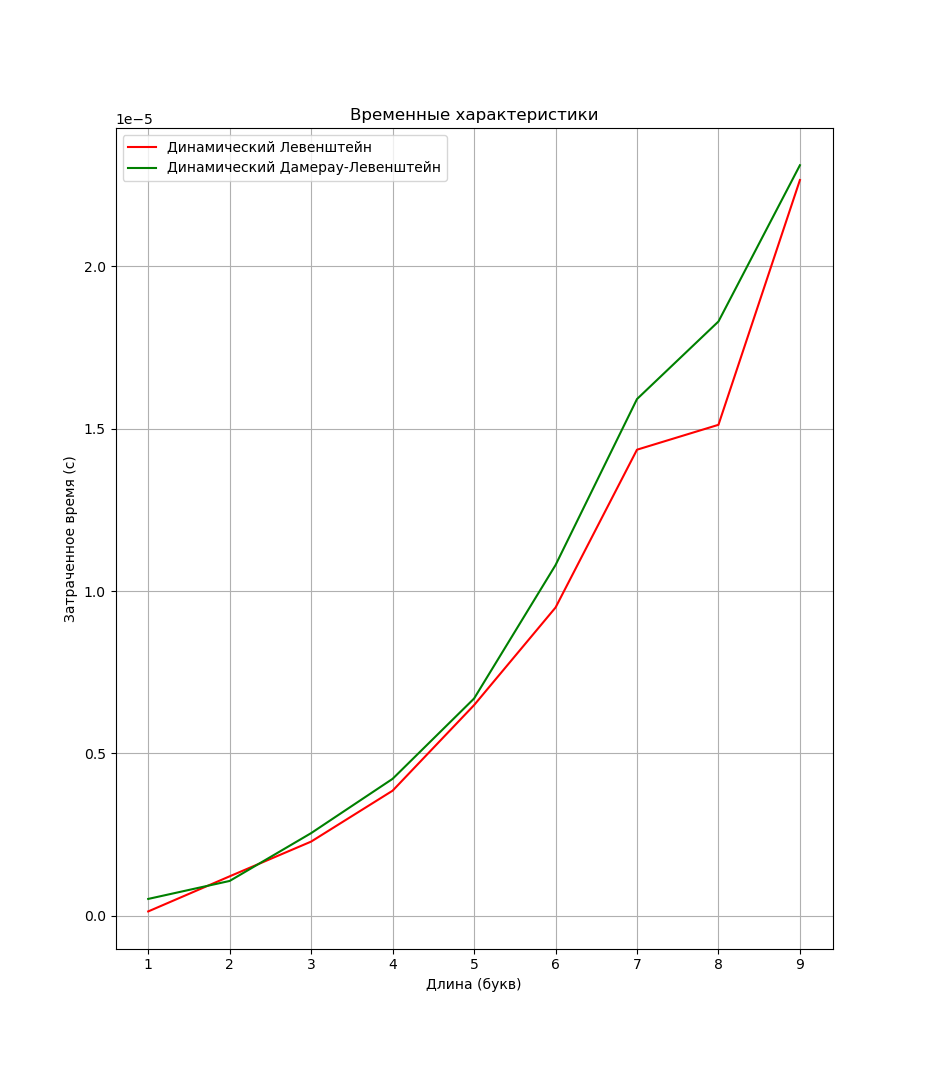
\includegraphics[width=0.8\textwidth]{images/Figure_2}
    \caption{Временные показатели динамических алгоритмов Левенштейна и Дамерау-левенштейна}
    \label{fig:DvsD}
\end{figure}

\clearpage

На рисунке \ref{fig:ALLvsALL} показаны графики зависимости времени от количества символов
для всех реализаций алгоритмов нахождения расстояния Левенштейна и Дамерау-Левенштейна.
\begin{figure}[h]
    \centering
    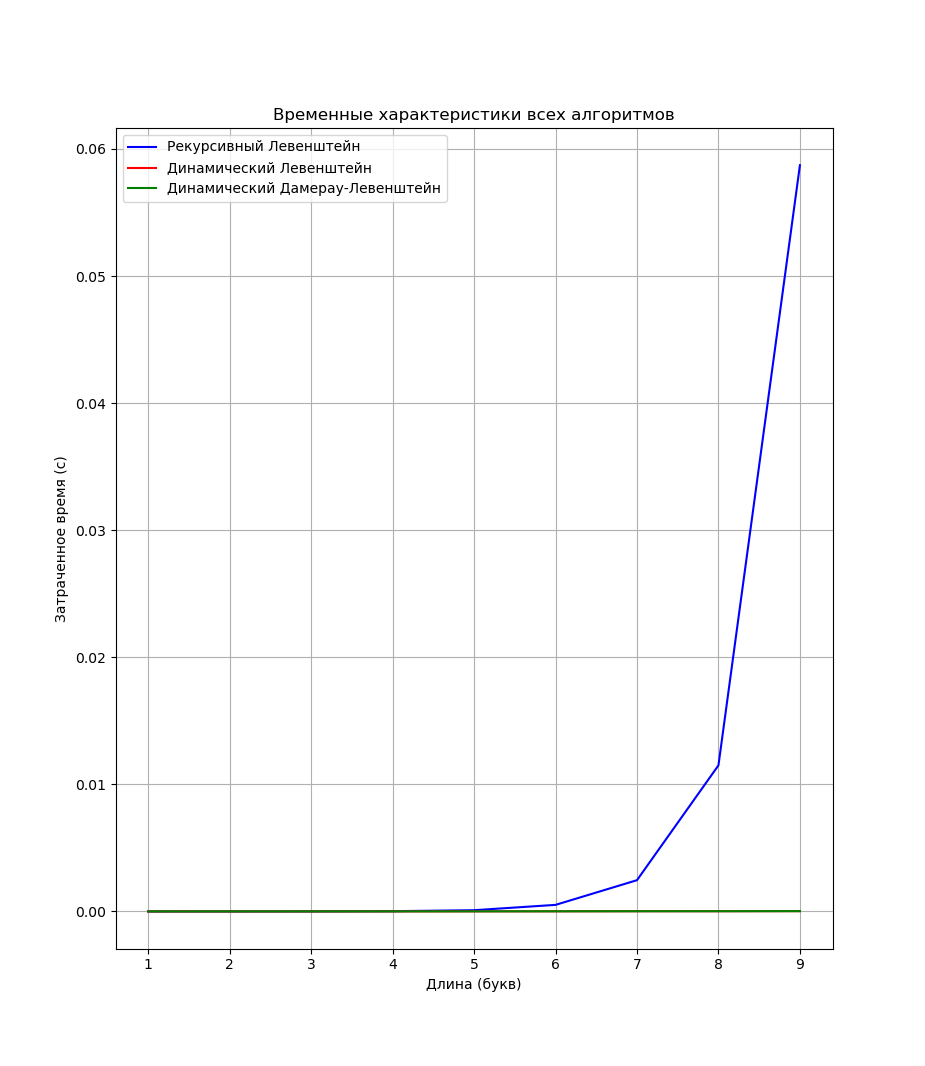
\includegraphics[width=0.8\textwidth]{images/Figure_3}
    \caption{Общие временные показатели}
    \label{fig:ALLvsALL}
\end{figure}

Наиболее эффективные реализации алгоритмы нахождения расстояния Левенштейна и
Дамерау-левенштейна  --- это те алгоритмы, где используется динамический подход, так
как в рекурсивном подходе идет повторный расчет. 

\section{Вывод}
Рекурсивный алгоритм, вычисляющий расстояние Левенштейна, работает по времени на
несколько порядков дольше, чем динамический вариант. Также стоит заметить, что
динамические алгоритмы вычисления расстояний Левенштейна и Дамерау-Левенштейна
сопостовимы между собой по времени выполнения и примерно равны.

Анализ расхода памяти показывает, что рекурсивный алгоритм имеет меньшие
требования к памяти по сравнению с алгоритмом, использующим динамическое
программирование. В случае динамического варианта алгоритма, считающего расстояние
Дамерау-Левенштейна, несмотря на добавление операции перестановки, потребление
памяти остается на уровне алгоритма, считающего расстояние Левенштейна, так
как не требуется дополнительное пространство для хранения результатов перестановок.



